\documentclass[letterpaper,10pt,a4paper]{article}
\usepackage{ulem}
\usepackage{url}

\usepackage{epsfig}
\usepackage{graphicx,color}% Include figure files
\usepackage{wrapfig,caption}
\usepackage{epstopdf}

\usepackage{fancyhdr,graphicx,epsfig,lastpage}
\usepackage{amsmath}
\usepackage{amssymb}

\usepackage{latexsym}
\usepackage[latin1,applemac]{inputenc}

%\usepackage{natbib}



\usepackage{mdwlist}
%\usepackage{enumitem}

%\usepackage[sort&compress,sectionbib]{natbib}
% \usepackage{german,isolatin1}
\usepackage{indentfirst}
%\usepackage{natbib}

\setlength{\parindent}{0in}
%\usepackage[superscript]{cite}

\usepackage{setspace} % Allows spacing of sections with \singlespacing and \doublespacing command

\oddsidemargin 0pt 
\evensidemargin 0pt 
\marginparwidth 68pt 
\marginparsep 10pt 
\topmargin 0pt 
\headheight 10pt 
\headsep 5pt

\voffset -40pt 
\footskip 35pt 
\textheight 23cm 
\textwidth 16.8cm 
\columnsep 10pt 
\columnseprule 0pt 
\sloppy 
%\frenchspacing

\linespread{1.27}

%\setlength{\parindent}{0pt} 
%\setlength{\parskip}{5pt plus 2pt minus 1pt}
%\renewcommand{\baselinestretch}{1.095} %{1.2} %{1.095}
%\clubpenalty=5000 \widowpenalty=5000
%\renewcommand{\footnoterule}{\vspace{0.5cm}%
%  \rule{2.5in}{0.4pt} \vspace{0.3cm}} \pagestyle{fancy}
%\renewcommand{\headrulewidth}{0.4pt} \lhead{Research Plan} \chead{}
%\rhead{\today} \renewcommand{\footrulewidth}{0.4pt} \lfoot{}
%\cfoot{\thepage /\pageref{LastPage}} \rfoot{}

%%%%%%%%%%%%%%%%%%%%%%%%%%%%%%%%%%%%%%%%%%%%%%%%%%%%%%%%%
% Main
%%%%%%%%%%%%%%%%%%%%%%%%%%%%%%%%%%%%%%%%%%%%%%%%%%%%%%%%%
\begin{document}
%\noindent
\begin{center}

  %\textbf{\Large Research Plan}\\[10mm]

%  \textbf{Title:}\\[5mm]
% \textbf{\Large Measuring Incentives for Attacks \& Security, }\\[4mm]
% \textbf{\Large and Managing Cyber Risk}\\ [10mm]

  %{\today}\\[85mm]

  %\textbf{PhD candidate:}\\
 % \textbf{\large Thomas Maillart}\\[10mm]

  %\textbf{Advisor:}\\
  %Prof. Dr. Didier Sornette\\
  %Chair of Entrepreneurial Risks\\
  %ETH Z\"urich (Swiss Federal Institute of Technology in Z\"urich)\\[5mm]

  % \textbf{Co-referee:}
  % \\[5mm]
  

\vspace{-0.5cm}
{\Large {\bf \textsc{Bringing Order to Wikipedia with Bi-Partite Network Rankings\\�}}}

\vspace{0.2cm}
{\large {\bf \textsc{Maximilian Klein, Thomas Maillart, John Chuang}}}
\vspace{0.15cm}
\end{center}

%Open source software has been one of the most successful incarnations of open innovation, providing considerable amount of software code as a public good for the development of reliable Internet and Web infrastructures, operating systems, and a broad range of applications.  Moreover, open source software (OSS) has inspired many initiatives beyond software development, such as Wikipedia  which combines (i) task self-selection and (ii) peer-review by participants.
\vspace{0.05cm}
%{\Large \bf Research Interests} \vspace{0.25cm}\\


%\clearpage
%\bibliography{../tmaillart.bib}
One of the very fundamental rules of peer-production in open collaboration projects is the ability for individuals to decide what tasks they want to 
take on \cite{benkler2002}. For instance, on Wikipedia some editors concentrate their efforts on a few selected articles, while others make little 
edits on a broader set of articles, and articles are likely to benefit from edits by more -- possibly expert -- contributors. The outstanding question 
is how individual contribution strategies are likely to influence the {\it expertise} of each editor, the {\it quality} of articles \cite{wang}, and ultimately the quality of the entire project \cite{geiger2013}. One way to tackle the problem consists in considering a project -- here a category of Wikipedia articles -- as a bi-partite network of articles and their related editors. Assessing the value of the two types of components of such a network has previously been undertaken in the context of macro-economics (ranking countries by the type of products they export) by Hidalgo and Haussmann \cite{hidalgo2009}, and by Caldarelli et al. \cite{caldarelli2012network}. The expertise of editors is assessed from the quantity and quality of articles they have edited. Conversely, the quality of an article depends on the number and the expertise of editors who have modified the article. Each iteration, information of article quality (resp. editor expertise) is recursively incorporated until the algorithm converges. The method is a two node types version of the Google pageRank algorithm \cite{page1999pagerank} and can be compared to a random walker jumping from one node to another type of node with some probability controlled by biased metrics of efferent node : $\alpha$ for the probability to jump from editor to article, and $\beta$ for the probability to jump from article to editor (see Figure \ref{fig1}A). 
\begin{figure}[h]
\centering
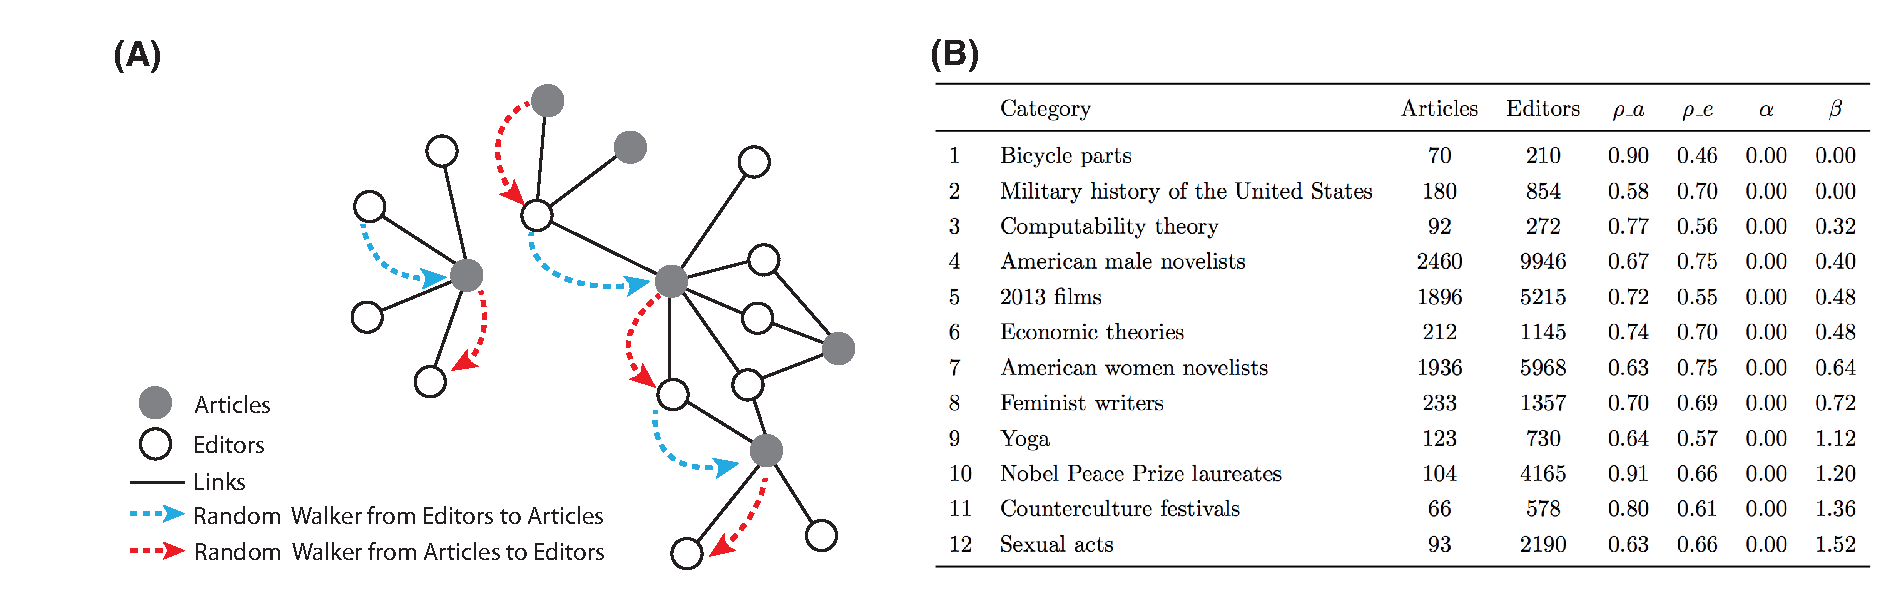
\includegraphics[width=0.8\columnwidth]{Figures/figure_abstract.eps}
\caption{{\bf (A)} Bi-partite network with Article and Editor nodes. Dashed arrows show how the random walker jumps from one node to another type of node with some probability controlled by the appropriately biased connectivity of the each node. {\bf (B)} Table shows the best rank-correlation $\rho_a$ and $\rho_e$ of the algorithm with the ground truth for each Wikipedia category, as well the value of the bias $\beta$.}
\label{fig1}
\end{figure}

The variables $\alpha$ and $\beta$ provide a direct measure of the ``value" of the number of editors per article and the ``value" of the number of articles per editor, respectively. Both $\alpha$ and $\beta$ are optimized to maximize the rank correlations of editors ($0.46 < \rho_e < 0.75 $) and articles ($0.57 < \rho_a < 0.91$) between the algorithm and ground-truth metrics obtained by state-of-the-art quality metrics of editors \cite{geiger2013} and articles \cite{wang}, for 12 categories of articles on Wikipedia. We find that the best value for $\alpha$ is $0$, while $0 \leqslant \beta \leqslant 1.52$ (c.f. Figure 1B). We find that the expertise of editors is concave increasing as a function of the number of articles they have edited for categories with $\beta > 1$ and decreasing when $0 < \beta < 1$. For two categories ({\it bicycle parts} and {\it Military history of the US}), $\beta = 0$, so the expertise of editors is a linear function of the number of articles they have edited. Regarding articles, the quality is a linear function of the number of editors, and a function of the expertise of these editors, which in turn varies depending on the values of $\beta$. For $\beta = 0$, the expertise of editors has no influence, while for $\beta > 0$, the expertise provided by editors decreases as a function of the number of articles they have edited. 




\clearpage
%Performing calculations on the bi-partite network as model has been proposed in Economics to rank countries and products \cite{hidalgo2009}, and the method has been shown to be able to predict GDP. \cite{caldarelli2012network}.
%
%In the Wikipedia bi-partite network, we adopt the premise that the quality of an editor depends on the size and quality of the portfolio of touched articles. And that the quality of an article depends on the size and quality of the log of touching editors. Although this many seem circular a solution is available \cite{caldarelli2012network}
%
%Therefore we borrow their quality metric $\mathbf{w^*}$ for editors $e$ and articles as $a$ defined by:
%\begin{equation}
%\begin{cases}
%w^{*}_{e} \sim k^{1-\beta}_{e} \langle k_{a}^{-\alpha}\rangle_e \\
%w^{*}_{a} \sim k^{1-\alpha}_{a} \langle k_{e}^{-\beta}\rangle_a
%\end{cases} \label{eqsim}
%\end{equation} 
%
%Where $k_e$ is the number of articles touched by editor $e$, and $k_a$  is number of editors touching article $a$. Similarly $\langle k_{a}^{-\alpha}\rangle_e$ is the arithmetic average of $k_{a}^{-\alpha}$ the articles touched by editor $e$, and $\langle k_{e}^{-\beta}\rangle_a$ is arithmetic average of $k_{e}^{-\beta}$ the editors touching article $e$.
%
%Meanwhile we calculate state of the art ground truth exogenous ranks $v_e$ and $v_a$ which are labour hours of editors \cite{geiger2013}, and a suite of text analysis measures on articles \cite{wang}.
%
%----------
%
%Despsite the calculation appearing to be circular, it can be solved recursively. The quality of editors and articles can be viewed as a heatmap of most touched nodes on a random walk along the bi-partite network of editors and articles shown on Figure \ref{fig1}A. We can tune our models by the probabilities of landing on more ubiquitously edited articles, and more diversified editors, by variables we call $\alpha$ and $\beta$. Therefore when we maximize the correlations between the ranking given by the bi-partite model, and standard metrics of editor and article quality, we find the most characteristic measurements of a category given by $\alpha$ and $\beta$.
%----------
%
%
%
%
%
%We calibrate our model by finding values of $\alpha$ and $\beta$ that maximally correlate the rank produced by the bi-partite network and the exogenous ranks. We achieve high correlations around $0.7$  which means that we may turn to see what values of  $\alpha$ and $\beta$ caused this correlation and what it means as an exhibited behaviour of those categories.
%
%The most notable result is in correlating article rankings there is a very clear solution space along $\alpha = 0$ across all categories. Namely that article quality is mostly explained as a simple count of contributing editors.  
%
%We would like to find solutions which maximize editor and article ranking correlations simultaneously so we could make a complete statement about all aspects of the category. We search the solution space of editor ranking correlations along $\alpha = 0$, whose interpretation in editor ranking is that the quality of articles in their edit portfolio is inconsequential. For each category we find different maximizing values of $\beta$, which is a measure of importance of portfolio size. High $\beta$ means that portfolio size is less important for successful editors, and vice-versa, low $\beta$ means article diversity counts more.
%
%Looking at \ref{fig1}B, we find interesting extremes. The best editors in {\it Category:Military history of the US} - a category known for being very competitive -  are characterized by emphasizing their article portfolio size. On the other end, the editors in {\it Category:Sexual acts} - a taboo subject where much editing could be considered perverse - are characterized by de-emphasizing their portfolio size in the category.
%
%Now if we allow that portfolio size, the number of articles that an editor has touched, is a proxy for a power-user, then our $\beta$ measure is an indicator for power-user domination of a category. Therefore using this method, open collaborations online can detect the importance of power-users to a specific project. 
%
%
%%While wikiRanks incorporates only bi-partite links input information, we find high rank correlations ($\rho = 0.7\pm0.1$) with usual Wikipedia editors' expertise and articles' quality metrics. The wikiRanks algorithm also provides deep insights on the structure of online collaboration. We find that editors in some categories of Wikipedia articles achieve more quality with a large number of editors per article, while for other categories, quality is more achieved as a result of expertise of editors.
%




%\clearpage
\vspace{1cm}
\bibliographystyle{abbrv}
\bibliography{sigproc,tmaillart}  


\end{document}
